% ============================================================================================================
\chapter{Audit de la version 0.6}\label{ch:audit}
% ============================================================================================================

La version 0.6 du modèle, documentée dans le rapport du 18 novembre 2026, est un modèle macroéconométrique de demande
(équations à correction d'erreur estimées sur données françaises) couplé à un tableau entrées-sorties à 64 produits et
25 branches, à un module de retraites (M9), à une microsimulation des ménages fondée sur OpenFisca-France (M10), à un
module de zone euro (M11), aux comportements des hauts revenus (M13) et à une hétérogénéité des propensions à
consommer (M14). Cette phase ne cherche pas à confirmer ses conclusions. L'audit a commencé par une question simple,
posée au modèle lui-même : \emph{que se passe-t-il si l'économie française devient moins productive ?}

\section{Le test qui a révélé le défaut}

Deux chocs d'offre défavorables ont été simulés sur la trajectoire de référence de la v0.6 (instantané figé du code,
script \code{phase3/diagnostic\_fermeture.py}, résultats \code{phase3/resultats/diagnostic\_v06.json}) :
\begin{itemize}
\item un ralentissement de la productivité du travail de 0,3 point par an à partir de 2028 ;
\item une baisse de la population active de 0,2 \% par an (choc démographique).
\end{itemize}
Un modèle économique cohérent doit conclure que ces chocs appauvrissent le pays : le PIB baisse, les recettes
publiques suivent, la dette rapportée au PIB augmente. Le tableau~\ref{tab:audit} montre ce que donnait la v0.6.

\begin{table}[h]\centering\small
\caption{Effets de deux chocs d'offre défavorables dans la v0.6 (écarts à la référence en 2037). Simulations exécutées.}\label{tab:audit}
\begin{tabular}{lrrrrrr}\toprule
Choc & PIB & Emploi & Chômage & Prix & Dette/PIB & Solde/PIB\\ \midrule
Productivité $-0{,}3$ pt/an & $-0{,}87$ \% & $+0{,}47$ \% & $-0{,}43$ pt & $+1{,}67$ \% & $-4{,}5$ pt & $+0{,}40$ pt\\
\quad idem, sans fermeture ($\rho=0$) & $-0{,}11$ \% & --- & $-1{,}06$ pt & --- & $-8{,}4$ pt & ---\\
Population active $-0{,}2$ \%/an & $-1{,}13$ \% & --- & $-0{,}95$ pt & $+1{,}45$ \% & $-1{,}37$ pt & ---\\ \bottomrule
\end{tabular}
\end{table}

\begin{limites}[Le paradoxe]
Dans la v0.6, une économie moins productive avait \emph{moins} de chômage et \emph{moins} de dette. Le PIB ne baissait
que de 0,9 \% en 2037, alors que la capacité de production (PIB potentiel) aurait dû baisser d'environ 2,7 \%. Ce
résultat contredit la théorie économique et l'expérience : le ralentissement de la productivité après 2008 s'est
accompagné d'une hausse, non d'une baisse, du ratio de dette.
\end{limites}

\section{Remonter à la cause, et non corriger le symptôme}

L'enchaînement a été vérifié équation par équation.
\begin{enumerate}
\item \textbf{Il n'y avait pas de PIB potentiel.} La production était déterminée par la demande. L'offre
n'intervenait que par le taux d'utilisation des capacités de l'industrie.
\item \textbf{Le choc de productivité n'entrait que dans l'équation d'emploi.} Pour produire autant, il fallait plus
de salariés : l'emploi montait, le chômage baissait. De plus, la correction d'erreur de cette équation effaçait le
choc en quelques années, parce que la cible de long terme ne l'incluait pas.
\item \textbf{La fermeture agissait sur le chômage, pas sur la production.} Le mécanisme qui ramène l'économie vers
son équilibre de moyen terme (politique monétaire, crédit, confiance : canaux non modélisés explicitement) voyait un
chômage « trop bas » et réduisait la demande, mais ne voyait jamais que la capacité de produire avait baissé.
\item \textbf{La boucle prix-salaires gonflait le PIB nominal.} Les coûts unitaires augmentaient, les prix aussi ; le
PIB en valeur augmentait (+1,7 \% en 2037) alors que le PIB en volume baissait. Le ratio dette/PIB, calculé en
valeur, baissait mécaniquement.
\item \textbf{Le chômage structurel était incohérent avec la référence} (7,5 \% dans la fermeture, 7,0 \% dans la
trajectoire calée), ce qui imposait un biais permanent compensé par les termes de calage.
\item \textbf{Il n'y avait pas de stabilisateur chômage} : la dépense d'indemnisation ne dépendait pas du nombre de
chômeurs, contrairement à ce qu'affirmait la documentation du code.
\item \textbf{Il n'y avait pas de courbe de Phillips sur les prix hors industrie}, ni d'effet des tensions de
capacité sur les importations.
\end{enumerate}

\begin{resultat}
La cause structurelle est l'absence de bloc d'offre : sans PIB potentiel, le modèle ne pouvait pas distinguer une
baisse de la demande d'une baisse de la capacité de produire. Les autres défauts (fermeture sur le chômage, choc de
productivité effacé, stabilisateur absent) amplifiaient ce défaut central.
\end{resultat}

% ============================================================================================================
\chapter{Faiblesses structurelles et priorités}\label{ch:faiblesses}
% ============================================================================================================

L'audit ne s'est pas limité au paradoxe des chocs d'offre. Chaque mécanisme de la v0.6 a été confronté à la
littérature empirique. Le tableau~\ref{tab:defauts} recense les défauts identifiés, leur conséquence sur les
résultats, leur priorité et le traitement retenu. Le détail figure dans \code{doc/15\_audit\_v06\_phase3.md}.

\begin{table}[htbp]\centering\scriptsize
\caption{Inventaire des défauts de la v0.6 et traitement en v0.7.}\label{tab:defauts}
\begin{tabularx}{\linewidth}{@{}rL L l L@{}}\toprule
\# & Défaut & Conséquence & Priorité & Traitement v0.7\\ \midrule
1 & Fermeture sur le chômage, pas de PIB potentiel & Paradoxe des chocs d'offre & Critique & PIB potentiel Cobb-Douglas ; fermeture sur l'écart de production ; anticipation\\
2 & Chômage structurel incohérent avec la référence & Biais permanent & Critique & Trajectoire 7,5 → 7,0 \% (2026-2031)\\
3 & Choc de productivité effacé par la correction d'erreur de l'emploi & Choc transitoire au lieu de permanent & Critique & Choc cumulé dans la cible de long terme\\
4 & Emploi proportionnel à la production, même quand le capital augmente & Chômage durablement trop bas après un investissement & Élevée & Terme d'approfondissement du capital\\
5 & Indemnisation chômage indépendante du chômage & Pas de stabilisateur & Élevée & Dépense proportionnelle aux chômeurs\\
6 & Pas de Phillips prix hors industrie ; importations insensibles aux tensions & Surchauffe sans inflation & Élevée & $\kappa = 0{,}10$ ; $\mu = 0{,}3$\\
7 & TVA répercutée à 80 \%, de façon symétrique et immédiate & Surestime l'effet des baisses & Élevée & Répercussion asymétrique et étalée\\
8 & IS sans transfert de bénéfices & Surestime le rendement des hausses & Élevée & Semi-élasticité 0,8 (groupes)\\
9 & Offre de travail exogène (RSA et prime d'activité au même effet) & Faux pour les prestations & Élevée & Module M15 (OpenFisca)\\
10 & Bénéfices conservés sans usage & Pas de canal de trésorerie & Moyenne & Réinvestissement de 10 \%\\
11 & Pas de délocalisation liée à l'énergie & Chocs énergie sous-estimés pour l'industrie lourde & Moyenne & Élasticité 0,15 (4 produits)\\
12 & Effet de l'assurance chômage sur le chômage structurel arbitraire & Non documenté & Moyenne & Élasticité de durée 0,3\\
13 & Pas d'épargne de précaution ni d'effet du taux réel & Multiplicateurs trop stables & Moyenne & $\psi_u = 0{,}3$ ; $\psi_r = 0{,}2$\\
14 & Salaires symétriques & Désinflation trop facile en récession & Moyenne & Rigidité à la baisse (× 0,5)\\
15 & Dépense publique indifférenciée & Pas de leviers d'offre (R\&D, formation) & Moyenne & Deux leviers exploratoires\\
16 & Microsimulation statique & Pas d'effets dynamiques par décile & Moyenne & Partiel (M15) ; groupes de ménages\\
17 & Autres dépenses ∝ PIB nominal & Masque une partie de l'effet des chocs & Faible & Conservée et documentée\\
18 & Pas de bilans patrimoniaux & Pas d'effets de richesse & Faible-moyenne & Non traité\\ \bottomrule
\end{tabularx}
\end{table}

Deux défauts (n\textsuperscript{os}~3 et~4) n'ont pas été trouvés par l'audit initial, mais par les tests de la
nouvelle version : après l'introduction du PIB potentiel, la production suivait bien le potentiel, mais le chômage
s'écartait durablement de son niveau structurel. C'est l'un des intérêts d'un bloc d'offre explicite : il rend
visibles les incohérences entre équations.

% ============================================================================================================
\chapter{La nouvelle architecture comportementale}\label{ch:architecture}
% ============================================================================================================

\section{Principe}

La v0.7 conserve le cœur de la v0.6 : les équations de court terme restent estimées sur données françaises, et le
tableau entrées-sorties répartit la demande entre branches. Elle ajoute trois éléments.
\begin{enumerate}
\item \textbf{Un bloc d'offre} : à chaque date, le modèle calcule ce que l'économie peut produire sans tensions
(PIB potentiel), à partir du capital, de la population active, du chômage structurel et de la productivité. Il en
déduit l'écart de production, qui alimente les prix, les importations et la fermeture.
\item \textbf{Des comportements explicites} : ménages (épargne de précaution, effet du taux d'intérêt, offre de
travail par configuration familiale), entreprises (transfert de bénéfices, trésorerie, délocalisation énergétique,
répercussion de la TVA, R\&D), prix et salaires (rigidité à la baisse, Phillips), stabilisateur chômage.
\item \textbf{Trois niveaux de comportement} (bas, central, haut) pour chaque paramètre incertain, sélectionnables
dans le simulateur (hypothèse \code{comportements\_v07}).
\end{enumerate}

\section{Court terme et moyen terme}

Le modèle combine deux logiques. À court terme (1 à 3 ans), la demande domine : une hausse des dépenses publiques
augmente la production, une hausse d'impôt la réduit. À moyen terme (5 à 10 ans), l'offre domine : la production
rejoint le potentiel, qui dépend du travail disponible, du capital et de la productivité. Une mesure qui ne fait que
stimuler la demande a donc un effet qui s'estompe ; une mesure qui augmente le potentiel (allongement de la vie
active, durée du travail, offre de travail, investissement productif) a un effet durable.

\begin{encadre}{Pourquoi une « anticipation » ?}
Une fermeture fondée uniquement sur l'écart de production observé laisse un écart permanent quand le potentiel baisse
progressivement (un choc de productivité de 0,3 point par an, cumulé sur 20 ans) : le mécanisme de rappel court
toujours derrière la cible. La v0.7 ajoute donc un terme par lequel la demande des ménages et des entreprises
s'ajuste à la révision du potentiel (revenu permanent). Son intensité ($\theta = 1{,}5$) a été choisie par
simulation pour que l'écart de production se referme en moins de dix ans après un choc d'offre, sans dépassement
(§\,\ref{sec:fermeture}). C'est une hypothèse de modélisation \preuve{H}, testée à 1,0 et 2,0.
\end{encadre}

\section{Ménages}

\begin{itemize}
\item \textbf{Consommation} : équation estimée de la v0.6, plus deux termes : $-0{,}3$ \% de consommation par point de
hausse du chômage (épargne de précaution) et $-0{,}2$ \% par point de hausse du taux d'intérêt réel.
\item \textbf{Offre de travail (nouveau module M15)} : pour cinq configurations familiales (personne seule, parent
isolé, couple sans enfant avec conjoint en emploi, couple avec enfants avec conjoint en emploi ou sans emploi), deux
niveaux de salaire (0,5 et 1 SMIC) et le taux marginal à 1,5 SMIC, OpenFisca-France calcule le gain financier à
travailler et le taux marginal effectif, avant et après la mesure. La participation réagit au gain (élasticité 0,2),
les heures au taux marginal (élasticité 0,1). Les effectifs viennent du recensement.
\item \textbf{Hétérogénéité} : les propensions à consommer par décile (M14) et la microsimulation (M10) sont
inchangées ; la microsimulation publie désormais les résultats par âge, catégorie sociale, région et configuration
familiale.
\end{itemize}

\section{Entreprises}

\begin{itemize}
\item \textbf{Investissement} : l'équation estimée (accélérateur, coût d'usage) est complétée par un canal de
trésorerie : 10 \% des bénéfices conservés sont investis. Une baisse d'impôt sur les sociétés n'augmente
l'investissement que par ce canal et par le coût d'usage ; elle n'est pas supposée « automatiquement » investie.
\item \textbf{Impôt sur les sociétés} : la base imposable des groupes (la moitié de l'IS) se déplace vers l'étranger
quand le taux augmente (semi-élasticité 0,8).
\item \textbf{Prix et marges} : la TVA est répercutée à 95 \% en cas de hausse, à 50 \% en cas de baisse (taux
normal) ; la part non répercutée accroît les marges, donc les profits.
\item \textbf{Délocalisation} : les importations des quatre industries les plus intensives en énergie augmentent
quand le prix relatif de l'énergie augmente.
\item \textbf{R\&D} : chaque euro d'aide entraîne 0,7 euro de R\&D privée supplémentaire ; le stock de R\&D augmente la
productivité (élasticité 0,08) avec deux ans de délai. Levier exploratoire.
\end{itemize}

\section{Couplage micro-macro}

Le couplage reste séquentiel (la microsimulation calcule les effets statiques d'une mesure sur les revenus des
ménages ; le modèle macroéconomique les reçoit comme un choc de revenu, corrigé de l'hétérogénéité des propensions à
consommer), avec deux ajouts : l'offre de travail calculée par M15 modifie la population active et les heures du
modèle macroéconomique (montée en charge sur deux ans), et le module de retraites M9 modifie la population active et
donc le PIB potentiel. La figure~\ref{fig:archi} résume l'architecture.

\begin{figure}[htbp]\centering
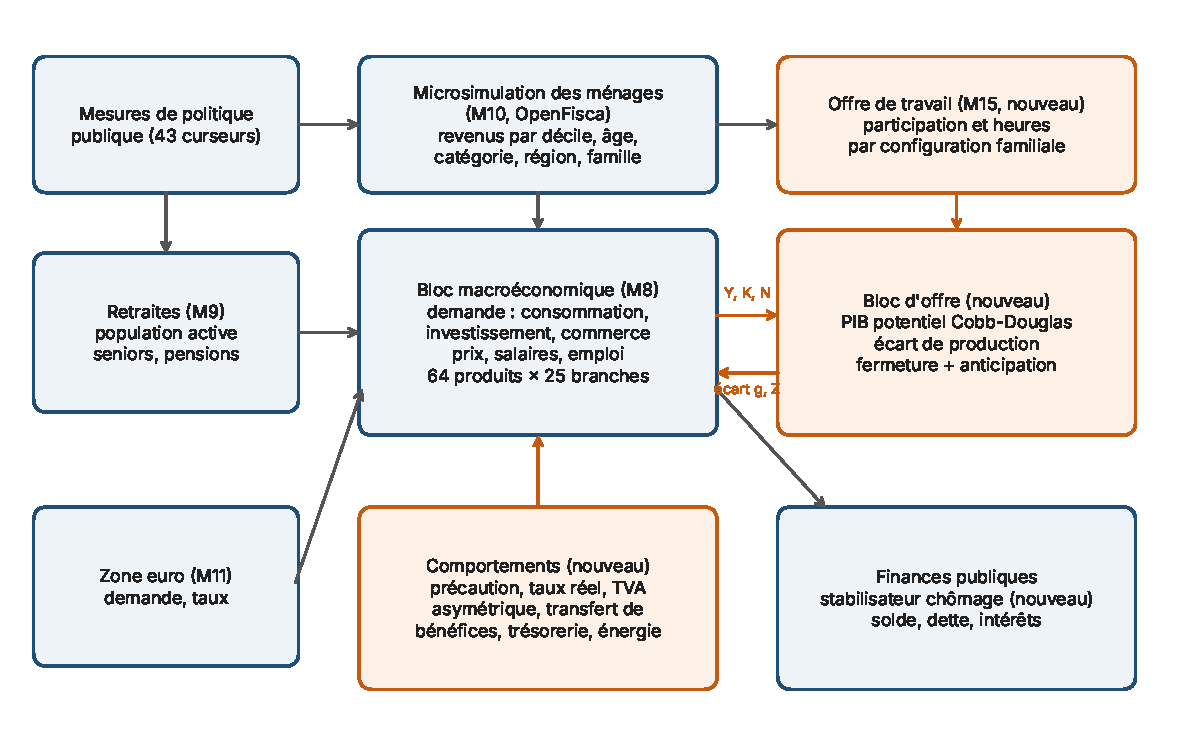
\includegraphics[width=\linewidth]{architecture_v07.pdf}
\caption{Architecture de la v0.7. En orange, les éléments nouveaux.}\label{fig:archi}
\end{figure}

% ============================================================================================================
\chapter{Équations et paramètres}\label{ch:equations}
% ============================================================================================================

\section{Bloc d'offre et fermeture}\label{sec:fermeture}

Le PIB potentiel suit une fonction de production Cobb-Douglas à rendements constants :
\begin{equation}
\ln Y^*_t = \mathrm{pgf}_t + \alpha \ln K_{t-1} + (1-\alpha)\ln N^*_t + \sum_{s\le t}\pi_s,
\qquad N^*_t = PA_t\,(1-u^*_t),
\end{equation}
où $K$ est le capital des branches marchandes, $PA$ la population active, $u^*$ le chômage structurel, $\pi$ les chocs
de productivité et $\alpha = 0{,}35$ la part du capital. La productivité globale des facteurs $\mathrm{pgf}_t$ est
celle qu'implique la référence calée, de sorte que l'écart de production de la référence vaut $-1{,}5\,(u-u^*)$ (loi
d'Okun) : la nouvelle fermeture ne modifie pas la référence (écart maximal de chômage entre les deux fermetures :
$10^{-5}$ point).

L'écart de production $g_t = \ln Y_t - \ln Y^*_t$ commande un supplément de demande intérieure $Z_t$ (60 \% en
consommation, 40 \% en investissement) :
\begin{equation}
Z_t = Z_{t-1} - \rho\, g_{t-1} - a\,(g_{t-1}-g_{t-2}) + \theta\,(\ln Y^*_{t-1}-\ln Y^{*,\mathrm{ref}}_{t-1}),
\end{equation}
avec $\rho = 0{,}15$, $a = 0{,}3$ et $\theta = 1{,}5$. Le terme en $\rho$ ramène progressivement la production vers le
potentiel ; le terme en $a$ amortit les oscillations ; le terme en $\theta$ représente l'anticipation.

\paragraph{Prix, importations.} L'équation de prix de la valeur ajoutée des branches hors industrie reçoit
$+\kappa\,g_{t-1}$ ($\kappa = 0{,}10$) ; celle des importations $+\mu\,(g_{t-1}-g_{t-2})$ ($\mu = 0{,}3$).

\paragraph{Emploi.} La cible de long terme de l'équation d'emploi de chaque branche devient
\begin{equation}
n^* = q - \sigma\,(w-p) - \gamma t - \sum_{s<t}\pi_s + \frac{\alpha}{1-\alpha}\,(\Delta q - \Delta k),
\end{equation}
où $\Delta q$ et $\Delta k$ sont les écarts (en log) du PIB et du capital marchand à la référence. Le dernier terme
assure qu'une production accrue par le seul capital ne crée pas d'emplois au même rythme que la production.

\section{Comportements}

\begin{align}
\Delta \ln C_t &= \text{(équation v0.6)} - \psi_u\,\Delta u_t - \psi_r\,\Delta r_t\\
\Delta \ln W_t &= \text{(équation v0.6)} + \lambda\,\phi(u_t - u^*_t), \quad \lambda = 0{,}5 \text{ si } u_t>u^*_t,\ 1 \text{ sinon}\\
IS_t &= IS_0\,\frac{EBE_t}{EBE_0}\,\frac{\tau_t}{\tau_0}\left[1 - m\left(1-e^{-\varepsilon(\tau_t-\tau_0)/100}\right)\right]\\
I_t &= \text{(équation v0.6)} + \vartheta\,\Pi^{\mathrm{conservés}}_t/p^I_t\\
\Delta PA_t &= \sum_{f}\eta^{\mathrm{ext}} N_f\, \Delta\ln(\text{gain à l'emploi})_f,
\qquad \Delta H_t = \sum_f \eta^{\mathrm{int}} N_f\,\Delta \ln(1-\mathrm{TME})_f
\end{align}

Les notations et valeurs sont données au tableau~\ref{tab:param}.

\section{Paramètres}

\begin{table}[htbp]\centering\scriptsize
\caption{Paramètres de comportement de la v0.7 : valeurs basse, centrale, haute et statut (E : estimé sur données
françaises ; L : littérature ; H : hypothèse ; X : exploratoire).}\label{tab:param}
\begin{tabularx}{\linewidth}{@{}l l r r r l L@{}}\toprule
Paramètre & Symbole & Basse & Centrale & Haute & Statut & Source\\ \midrule
Part du capital & $\alpha$ & --- & 0,35 & --- & E & Comptes nationaux\\
Rappel vers le potentiel & $\rho$ & 0 & 0,15 & 0,30 & H & Demi-vie 3-5 ans\\
Anticipation du potentiel & $\theta$ & 1,0 & 1,5 & 2,0 & H & Tests de simulation\\
Phillips prix & $\kappa$ & 0,05 & 0,10 & 0,18 & L & Banque de France\\
Importations / tensions & $\mu$ & --- & 0,3 & --- & H & Stabilité (§\,\ref{sec:fermeture})\\
Épargne de précaution & $\psi_u$ & 0,1 & 0,3 & 0,6 & L & Carroll ; épargne 2020-2021\\
Taux réel → consommation & $\psi_r$ & 0 & 0,2 & 0,5 & L & Havranek (2015)\\
Rigidité salariale à la baisse & $\lambda$ & 1,0 & 0,5 & 0,25 & L & Rigidité nominale\\
Semi-élasticité des bénéfices & $\varepsilon$ & 0,2 & 0,8 & 1,5 & L & Heckemeyer-Overesch ; Beer et al.\\
Part des groupes dans l'IS & $m$ & --- & 0,5 & --- & H & Concentration de l'IS\\
Trésorerie → investissement & $\vartheta$ & 0 & 0,10 & 0,30 & L & CICE ; dividendes 2013\\
Délocalisation énergétique & --- & 0 & 0,15 & 0,40 & L & Dussaux (2020) ; Marin-Vona\\
Participation & $\eta^{\mathrm{ext}}$ & 0,1 & 0,2 & 0,4 & L & Revue OFCE ; DARES\\
Heures & $\eta^{\mathrm{int}}$ & 0,05 & 0,1 & 0,2 & L & Idem\\
Assurance chômage → $u^*$ (pt/10 \%) & --- & 0 & 0,063 & 0,13 & L & Le Barbanchon et al.\\
Répercussion TVA hausse/baisse & --- & \multicolumn{3}{c}{0,95 / 0,50 (taux normal)} & L & Benzarti et al. (2020)\\
Additionnalité R\&D & --- & 0,3 & 0,7 & 1,2 & L/X & CNEPI (2021)\\
Élasticité au stock de R\&D & --- & 0,03 & 0,08 & 0,15 & L/X & Hall-Mairesse-Mohnen (2010)\\
Formation → $u^*$ (pt/Md€) & --- & 0 & 0,02 & 0,05 & X & Revue des évaluations\\ \bottomrule
\end{tabularx}
\end{table}

% ============================================================================================================
\chapter{Sources et calibrations}\label{ch:sources}
% ============================================================================================================

Chaque paramètre a été calibré selon la même démarche : recenser les estimations, vérifier leur champ (pays,
période, population, méthode), privilégier les études sur données françaises ou européennes, retenir une valeur
centrale et une fourchette, et indiquer la fragilité. Les paragraphes suivants résument les choix les plus
structurants.

\paragraph{Offre de travail.} Les revues de littérature trouvent des élasticités de participation très dispersées
(de 0,19 à 1,13 dans la revue de l'OFCE ; 27 études sur 35 au-dessus de 0,1). Les élasticités sont plus fortes pour
les mères isolées et les seconds apporteurs de revenu, plus faibles pour les hommes d'âge actif. La valeur centrale
0,2 est prudente ; la valeur haute 0,4 correspond aux populations les plus réactives. Pour les heures, l'élasticité
du revenu imposable en France est faible (0,02 en moyenne selon Cabannes, Houdré et Landais), d'où 0,1 en central.

\paragraph{Répercussion de la TVA.} L'étude de Benzarti, Carloni, Harju et Kosonen (\emph{Journal of Political
Economy}, 2020), sur des réformes européennes, montre que les hausses sont deux fois plus répercutées que les
baisses. En France, la baisse de TVA dans la restauration en 2009 a été très peu répercutée, les hausses de 2012 et
2014 l'ont été à environ 50 \% et 38 \%.

\paragraph{Impôt sur les sociétés.} Les méta-analyses donnent une semi-élasticité de la base aux taux d'environ 0,8
(Heckemeyer et Overesch), 1 à 1,5 (Beer, de Mooij et Liu), avec des estimations plus faibles sur données récentes
(Merlo et Wamser : 0,22). L'effet de l'IS sur l'investissement est faible en France : l'évaluation du CICE par
France Stratégie (2020) conclut à 100 000 emplois environ (160 000 dans l'estimation macroéconomique) mais à un effet
non concluant sur l'investissement ; la réforme de la fiscalité des dividendes de 2013 a fortement réduit les
dividendes sans effet sur l'investissement (Bach et al. ; Boissel et Matray).

\paragraph{Énergie.} Une hausse de 10 \% du prix de l'énergie réduit la consommation d'énergie de 6 \% et l'emploi
des entreprises concernées de 2 \%, sans effet net au niveau du secteur (Dussaux, OCDE, 2020) ; l'emploi
manufacturier baisse de 0,7 à 0,8 \% (Dechezleprêtre et al. ; Marin et Vona).

\paragraph{Assurance chômage.} Le Barbanchon, Rathelot et Roulet estiment sur données françaises une élasticité de la
durée de chômage à la durée potentielle d'indemnisation de 0,3.

\paragraph{R\&D.} L'évaluation du crédit d'impôt recherche (CNEPI, 2021) trouve 0,9 à 1,5 euro de R\&D par euro
d'aide pour les PME, sans effet de levier pour les grandes entreprises ; la valeur centrale de 0,7 en tient compte.

\paragraph{Courbe de Phillips.} La sensibilité de l'inflation à l'écart de production est faible dans les économies
avancées (0,18 point par point d'écart pour les États-Unis selon la Banque de France) ; la valeur centrale 0,10 est
plus basse pour tenir compte de l'ancrage des anticipations dans la zone euro.

\begin{limites}[Ce que les sources ne disent pas]
Presque toutes ces estimations viennent d'études quasi expérimentales sur une réforme, un secteur ou une période. Les
transposer à des réformes de grande ampleur, combinées entre elles, en équilibre général, est une extrapolation. C'est
pourquoi chaque résultat de ce rapport est présenté avec les comportements bas et haut.
\end{limites}
